\section*{Bài tập 5 --- Mô hình phân cụm}

%--------------------------------------------------------------------
\subsection*{Câu 5.1.1 --- K-means với $k=2$}

Cho các điểm trong $\mathbb{R}^2$:
\[
P_1=(1,1),\quad P_2=(2,1),\quad P_3=(4,3),\quad P_4=(5,4).
\]
Khởi tạo hai tâm $C_1^{(0)}=(1,1)=P_1$, $C_2^{(0)}=(5,4)=P_4$, và xét khoảng cách Euclidean.

\paragraph{Lần lặp đầu tiên (gán cụm theo hai tâm ban đầu).}
Với mọi điểm $P$, ta so sánh $d(P,C_1^{(0)})$ và $d(P,C_2^{(0)})$, chọn cụm có khoảng cách nhỏ hơn.

\begin{itemize}
  \item $P_1$: $d(P_1,C_1^{(0)})=0$, $d(P_1,C_2^{(0)})=\sqrt{(5-1)^2+(4-1)^2}=5$, chọn cụm $1$.
  \item $P_2$: $d(P_2,C_1^{(0)})=1$, $d(P_2,C_2^{(0)})=\sqrt{9+9}=3\sqrt2$, chọn cụm $1$.
  \item $P_3$: $d(P_3,C_1^{(0)})=\sqrt{(4-1)^2+(3-1)^2}=\sqrt{13}$,\\
        $d(P_3,C_2^{(0)})=\sqrt{(5-4)^2+(4-3)^2}=\sqrt2$, chọn cụm $2$.
  \item $P_4$: $d(P_4,C_1^{(0)})=5$, $d(P_4,C_2^{(0)})=0$, chọn cụm $2$.
\end{itemize}

Vậy sau bước gán đầu ta được hai cụm $\mathcal{S}_1^{(0)}=\{P_1,P_2\}$, $\mathcal{S}_2^{(0)}=\{P_3,P_4\}$.

\paragraph{Cập nhật tâm.}
Tâm mới là trung bình cộng toạ độ các điểm trong mỗi cụm:
\[
C_1^{(1)}=\frac{P_1+P_2}{2}=\Bigl(\tfrac32,\,1\Bigr),\qquad
C_2^{(1)}=\frac{P_3+P_4}{2}=\Bigl(\tfrac92,\,\tfrac72\Bigr)=(4{,}5,\;3{,}5).
\]

\paragraph{Vòng tiếp theo.}
Với $C_1^{(1)}, C_2^{(1)}$ như trên, một lần nữa tính khoảng cách đến từng tâm cho $P_1,\ldots,P_4$. Ta được phép phân cụm không đổi so với bước trước (hai cụm vẫn là $\{P_1,P_2\}$ và $\{P_3,P_4\}$).\\
Đồng thời, trung bình của các điểm trong hai cụm đó trùng hệt $C_1^{(1)}$ và $C_2^{(1)}$, nên không có chỗ chỉnh tâm nữa. Thuật toán \emph{dừng} và đây là kết quả cuối:
\begin{center}
\fbox{\parbox{0.92\linewidth}{
  \textbf{Cụm $1$:} $\{P_1,P_2\}$, \quad \textbf{tâm cuối:} $\bigl(\tfrac32,\,1\bigr)$.\\[2pt]
  \textbf{Cụm $2$:} $\{P_3,P_4\}$, \quad \textbf{tâm cuối:} $\bigl(\tfrac92,\,\tfrac72\bigr)$.
}}
\end{center}

%--------------------------------------------------------------------
\subsection*{Câu 5.1.2 --- K-means với $k=2$}

Các điểm:
\[
A(1,2),\quad B(2,1),\quad C(4,3),\quad D(5,4),\quad E(3,5),\quad F(6,5).
\]
Khởi tạo $C_1^{(0)}=(1,2)=A$, $C_2^{(0)}=(5,4)=D$.

\paragraph{(a) Gán cụm ở lần lặp đầu.}
Ta xét khoảng cách Euclidean đến hai tâm ban đầu:
\begin{itemize}
  \item $d(A,C_1^{(0)})=0$, $d(A,C_2^{(0)})=\sqrt{16+4}=2\sqrt5$, cụm $1$.
  \item $d(B,C_1^{(0)})=\sqrt2$, $d(B,C_2^{(0)})=3\sqrt2$, cụm $1$.
  \item $d(C,C_1^{(0)})=\sqrt{10}$, $d(C,C_2^{(0)})=\sqrt2$, cụm $2$.
  \item $d(D,C_1^{(0)})=2\sqrt5$, $d(D,C_2^{(0)})=0$, cụm $2$.
  \item $d(E,C_1^{(0)})=\sqrt{13}$, $d(E,C_2^{(0)})=\sqrt5$, cụm $2$.
  \item $d(F,C_1^{(0)})=\sqrt{34}$, $d(F,C_2^{(0)})=\sqrt2$, cụm $2$.
\end{itemize}
Vậy lần \emph{đầu} các cụm là $\mathcal{S}_1=\{A,B\}$, $\mathcal{S}_2=\{C,D,E,F\}$.

\paragraph{(b) Hai tâm sau khi cập nhật một lần.}
\begin{align*}
C_1^{(1)} &= \frac{A+B}{2} = \Bigl(\tfrac32,\,\tfrac32\Bigr) = (1{,}5,\;1{,}5),\\
C_2^{(1)} &= \frac{C+D+E+F}{4}
           = \Bigl(\tfrac{4+5+3+6}{4},\;\tfrac{3+4+5+5}{4}\Bigr)
           = \Bigl(\tfrac92,\,\tfrac{17}{4}\Bigr)=(4{,}5,\;4{,}25).
\end{align*}

\paragraph{(c) Tiếp tục đến hội tụ.}
Ở vòng tiếp theo, với $C_1^{(1)}=(\frac32,\frac32)$ và $C_2^{(1)}=(\frac92,\frac{17}{4})$, ta nhận lại đúng phép chia cụm như trên $\{A,B\}$ và $\{C,D,E,F\}$, và hai vector trung bình nhập vai các cụm này vẫn là $(\frac32,\frac32)$ và $(\frac92,\frac{17}{4})$, không đổi nữa. Thuật toán kết thúc!

\textbf{Kết luận:}
\begin{center}
\fbox{\parbox{0.92\linewidth}{
  Cuối cùng: cụm $1=\{A,B\}$, tâm $\bigl(\tfrac32,\,\tfrac32\bigr)$;\\
  cụm $2=\{C,D,E,F\}$, tâm $\bigl(\tfrac92,\,\tfrac{17}{4}\bigr)$.
}}
\end{center}

%--------------------------------------------------------------------
\subsection*{Câu 5.1.3 --- K-means với $k=2$ trên bảy đối tượng}

Các điểm có hai đặc trưng $x_1,x_2$:

\begin{center}
\begin{tabular}{@{}c cc@{}}
\toprule
Đối tượng & $x_1$ & $x_2$ \\
\midrule
$1$ & $1{,}0$ & $1{,}0$ \\
$2$ & $1{,}5$ & $2{,}0$ \\
$3$ & $3{,}0$ & $4{,}0$ \\
$4$ & $5{,}0$ & $7{,}0$ \\
$5$ & $3{,}5$ & $5{,}0$ \\
$6$ & $4{,}5$ & $5{,}0$ \\
$7$ & $3{,}5$ & $4{,}5$ \\
\bottomrule
\end{tabular}
\end{center}

Khởi tạo $C_1^{(0)}$ là đối tượng $1$, $C_2^{(0)}$ là đối tượng $4$.

\paragraph{Lần lặp $t=0$ (gán).}
Ta đối chiếu khoảng cách tới hai tâm $(1,1)$ và $(5,7)$; các đối tượng $1,2,3$ gần $(1,1)$ hơn, các đối tượng còn lại gần $(5,7)$ hơn.

Đặc biệt đối với đối tượng $3=(3,4)$:
\begin{align*}
d_3(C_1^{(0)}) &= \sqrt{(3-1)^2+(4-1)^2}=\sqrt{13},\\
d_3(C_2^{(0)}) &= \sqrt{(5-3)^2+(7-4)^2}=\sqrt{13}.
\end{align*}
Hai cự ly \emph{bằng nhau}; trong giải tay ta cố định quy tắc phá hoà là đặt vào cụm \emph{có chỉ số nhỏ hơn}, nên đối tượng $3$ được đặt vào cụm $1$.
Ta được hai cụm sau vòng đầu:
\[
\mathcal{S}_1^{(\mathrm{sau}\;0)}=\{1,2,3\},\qquad
\mathcal{S}_2^{(\mathrm{sau}\;0)}=\{4,5,6,7\}.
\]
Trung bình của các điểm trong hai cụm cho các tâm mới:
\[
C_1^{(1)}=\Bigl(\tfrac{11}{6},\;\tfrac{7}{3}\Bigr)\approx(1{,}833,\;2{,}333),\qquad
C_2^{(1)}=\Bigl(\tfrac{33}{8},\;\tfrac{43}{8}\Bigr)=(4{,}125,\;5{,}375).
\]

\paragraph{Lần lặp $t=1$ (gán lại).}
Với hai tâm vừa cập nhật, các đối tượng $\{1,2\}$ nằm gần $C_1^{(1)}$, các đối tượng $\{3,4,5,6,7\}$ nằm gần $C_2^{(1)}$.

Giờ hai cụm là $\{1,2\}$ và $\{3,4,5,6,7\}$.\\
Khi đó hai tâm cập nhật là:
\[
C_1^{(2)}=\Bigl(\tfrac54,\;\tfrac32\Bigr)=(1{,}25,\;1{,}5),\qquad
C_2^{(2)}=\Bigl(\tfrac{39}{10},\;\tfrac{51}{10}\Bigr)=(3{,}9,\;5{,}1).
\]

\paragraph{Lần lặp $t=2$.}
Một lần nữa, phép gán cụm không đổi so với bước trước, và hai vector trung bình trùng với $C_1^{(2)},C_2^{(2)}$, nên thuật toán dừng.

\textbf{Tóm tắt trạng thái các cụm theo từng vòng (theo thứ tự đã trình bày):}
\begin{center}
\begin{tabular}{@{}lll@{}}
\toprule
Sau vòng & Cụm $1$ & Cụm $2$ \\
\midrule
Sau lần gán đầu (theo $C_1^{(0)},C_2^{(0)}$) & $\{1,2,3\}$ & $\{4,5,6,7\}$ \\
Sau lần gán tiếp theo và kết quả cuối & $\{1,2\}$ & $\{3,4,5,6,7\}$ \\
\bottomrule
\end{tabular}
\end{center}

\textbf{Tọa độ tâm cuối cùng:}
\begin{center}
\fbox{\parbox{0.92\linewidth}{
$C_1^\star=\bigl(\tfrac54,\;\tfrac32\bigr)$,\quad
$C_2^\star=\bigl(\tfrac{39}{10},\;\tfrac{51}{10}\bigr)$.
}}
\end{center}

%--------------------------------------------------------------------
\subsection*{Câu 5.2.1 --- Phân cụm phân cấp (single linkage)}

Cho ba điểm $A=(1{,}0,\;1{,}0)$, $B=(1{,}5,\;1{,}5)$, $C=(5{,}0,\;5{,}0)$ và xét khoảng cách Euclidean giữa các điểm đơn lẻ.

Ta có các cự ly đối xứng:
\begin{align*}
d(A,B) &= \sqrt{(0{,}5)^2+(0{,}5)^2}=\sqrt{\tfrac12}=\tfrac{\sqrt2}{2}\approx 0{,}707,\\
d(A,C) &= \sqrt{4^2+4^2}=\sqrt{32}=4\sqrt2\approx 5{,}657,\\
d(B,C) &= \sqrt{(3{,}5)^2+(3{,}5)^2}=\sqrt{\tfrac{49}{2}}=\tfrac{7}{\sqrt2}=\tfrac{7\sqrt2}{2}\approx 4{,}950.
\end{align*}

\emph{Single linkage:} khoảng cách giữa hai cụm là \emph{cự ly nhỏ nhất} giữa một điểm thuộc cụm này và một điểm thuộc cụm kia.

\begin{enumerate}
  \item \textbf{Bước hợp nhất đầu tiên:} cự ly nhỏ nhất trong các cặp điểm là $d(A,B)=\sqrt2/2$, nên ghép $A$ và $B$ trước, độ cao nối trên dendrogram là $\sqrt2/2$.
  \item \textbf{Bước thứ hai:} xét cụm $\{A,B\}$ và điểm $C$. Theo single linkage,
  \[
  d(\{A,B\},C)=\min\{d(A,C),\,d(B,C)\}=\min\{4\sqrt2,\,\tfrac{7\sqrt2}{2}\}=\tfrac{7\sqrt2}{2},
  \]
  vì $\tfrac72<4$. Toàn bộ tập được gom lại ở cự ly $\tfrac{7\sqrt2}{2}$.
\end{enumerate}

\begin{figure}[htbp]
  \centering
  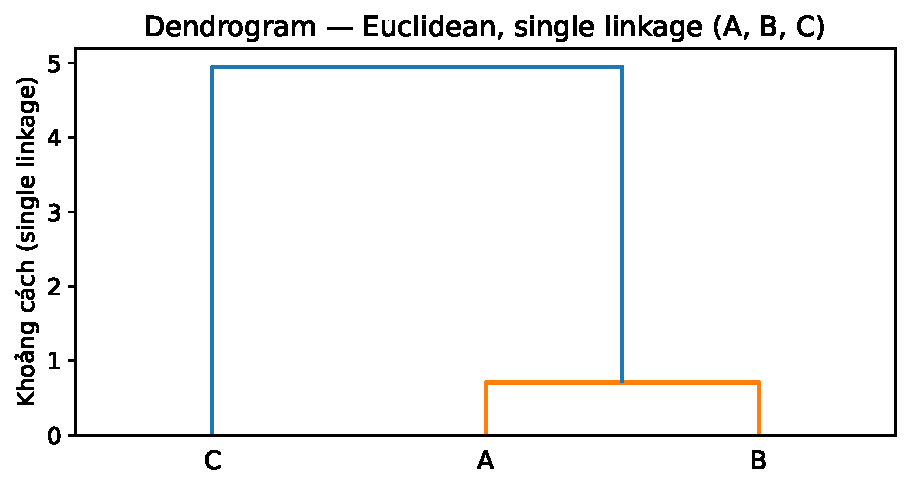
\includegraphics[width=0.88\linewidth]{figures/fig_dendrogram_abc.pdf}
  \caption{Dendrogram tương ứng với hai bước hợp nhất (single linkage).}
\end{figure}

%--------------------------------------------------------------------
\subsection*{Câu 5.2.2 --- Phân cụm phân cấp (single linkage)}

Cho $D=(3{,}0,\;4{,}0)$, $E=(4{,}0,\;4{,}0)$, $F=(3{,}0,\;3{,}5)$.

Ta có:
\begin{align*}
d(D,E) &= \sqrt{(4-3)^2+(4-4)^2}=1,\\
d(D,F) &= \sqrt{0^2+(0{,}5)^2}=0{,}5,\\
d(E,F) &= \sqrt{(4-3)^2+(4-3{,}5)^2}=\sqrt{1{,}25}=\tfrac{\sqrt5}{2}\approx 1{,}118.
\end{align*}

\begin{enumerate}
  \item \textbf{Bước $1$:} cự ly nhỏ nhất là $d(D,F)=0{,}5$, nên hợp nhất $D$ và $F$ trước (độ cao $0{,}5$).
  \item \textbf{Bước $2$:} giữa cụm $\{D,F\}$ và điểm $E$, ta áp dụng single linkage:
  \[
  d(\{D,F\},E)=\min\{d(E,D),\,d(E,F)\}=\min\{1,\,\tfrac{\sqrt5}{2}\}=1,
  \]
  vì $1<\sqrt5/2$. Ghép toàn bộ ở cự ly $1$.
\end{enumerate}

\begin{figure}[htbp]
  \centering
  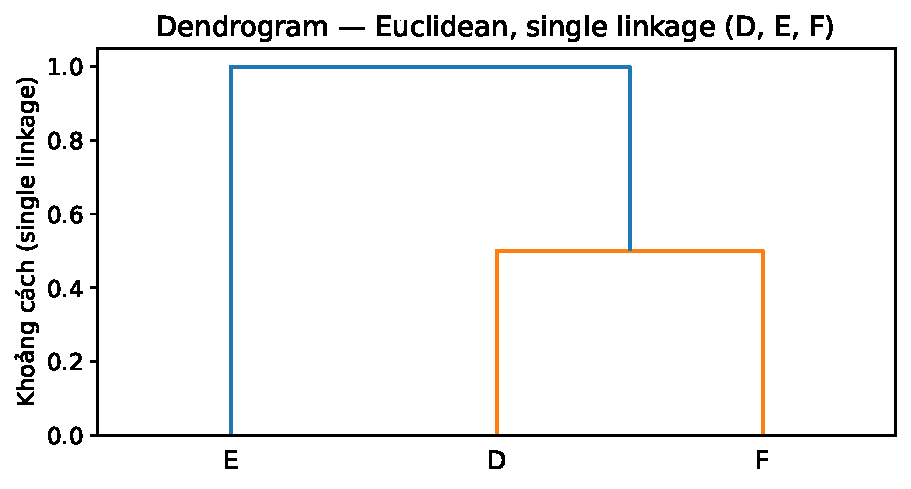
\includegraphics[width=0.88\linewidth]{figures/fig_dendrogram_def.pdf}
  \caption{Dendrogram cho ba điểm $D,E,F$ với single linkage.}
\end{figure}
